\section{Results and Discussions }
%\section{Expected Results}
Three similar motors were chosen at different stages of their useful life:
\begin{itemize}
	\item Motor1: New motor at max value of remaining useful life ie TIME = t
	\item Motor2: Motor at remaining useful life is approximately  t/2
	\item Motor3: Motor at remaining useful life = 0   
\end{itemize} 

Data collected was returned as in the table below, indexed in time series data points that can often illustrate trends or patterns in a more accessible, intuitive way.

\begin{figure}[!h]
	%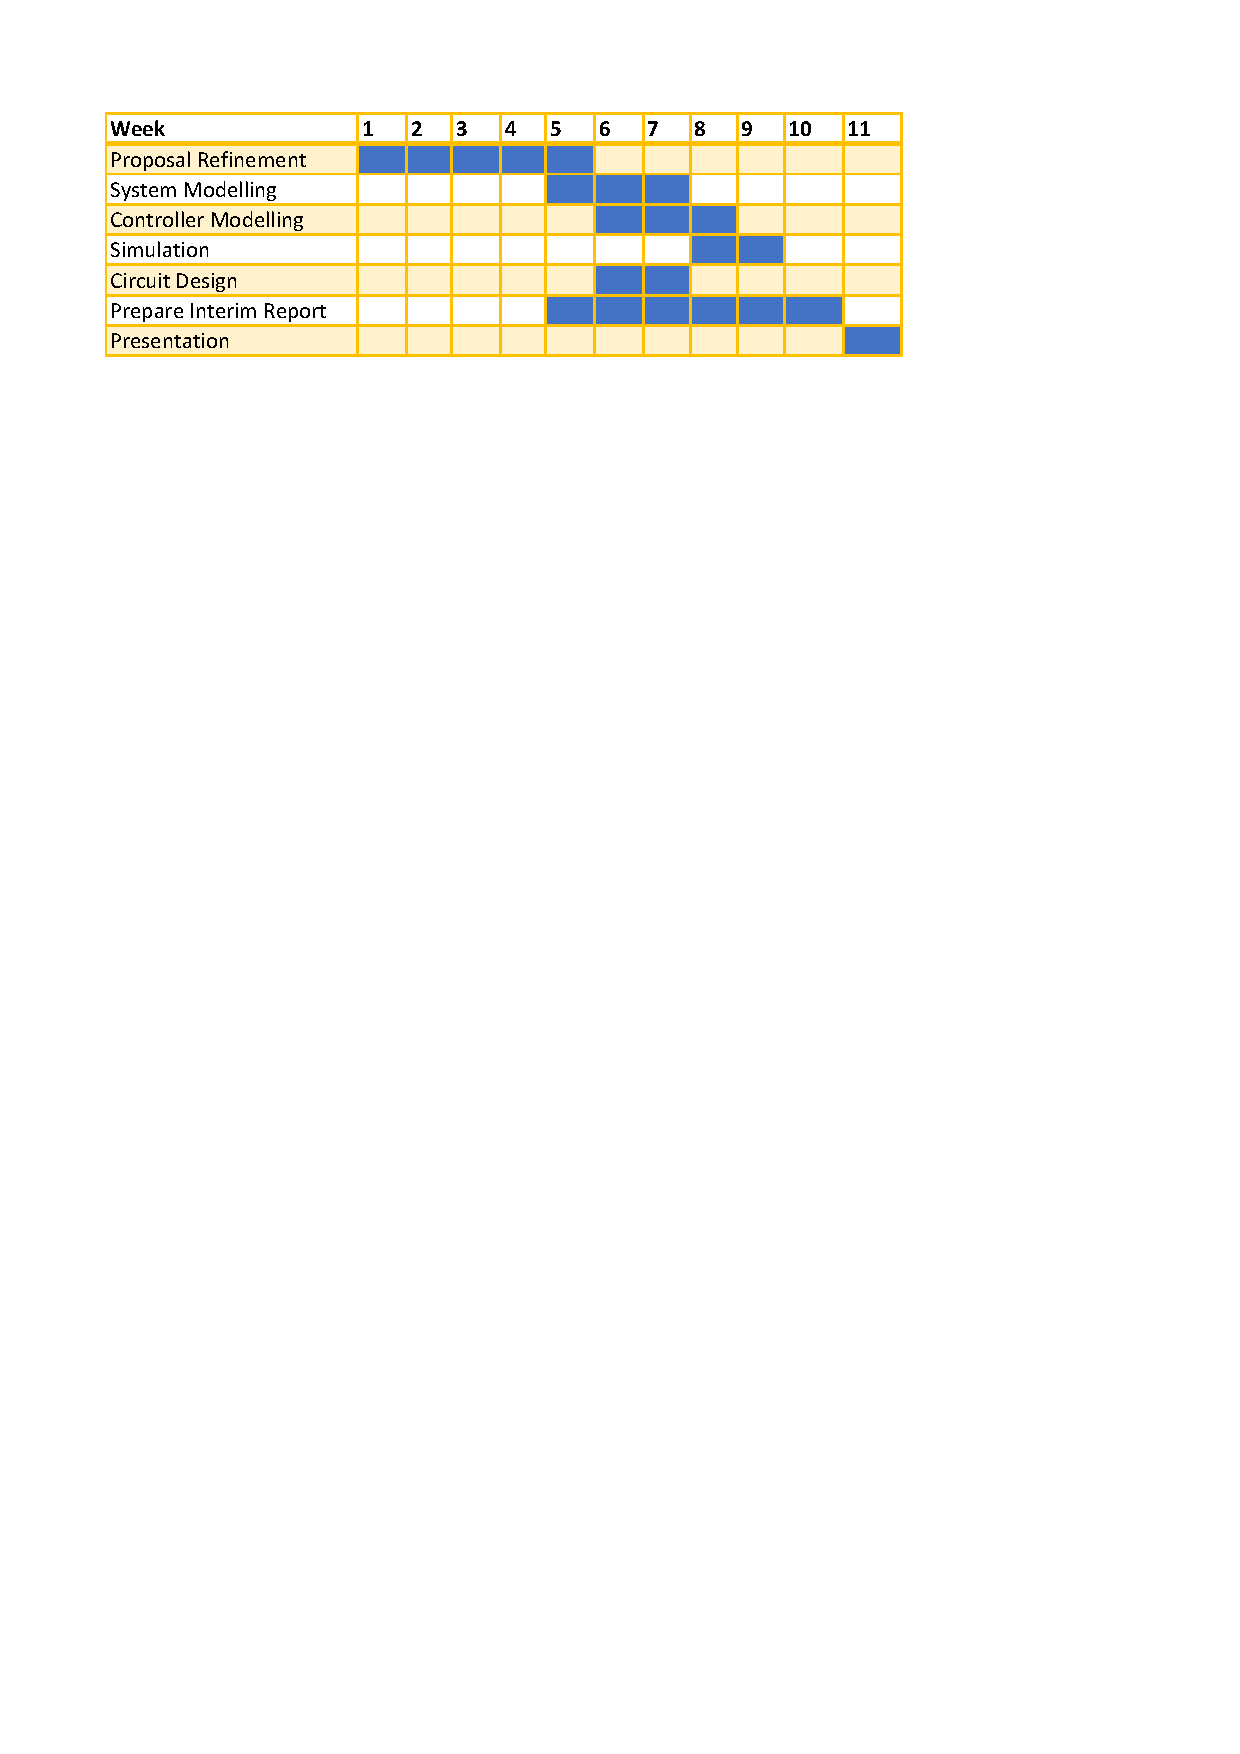
\includegraphics{Figures/workplan}
	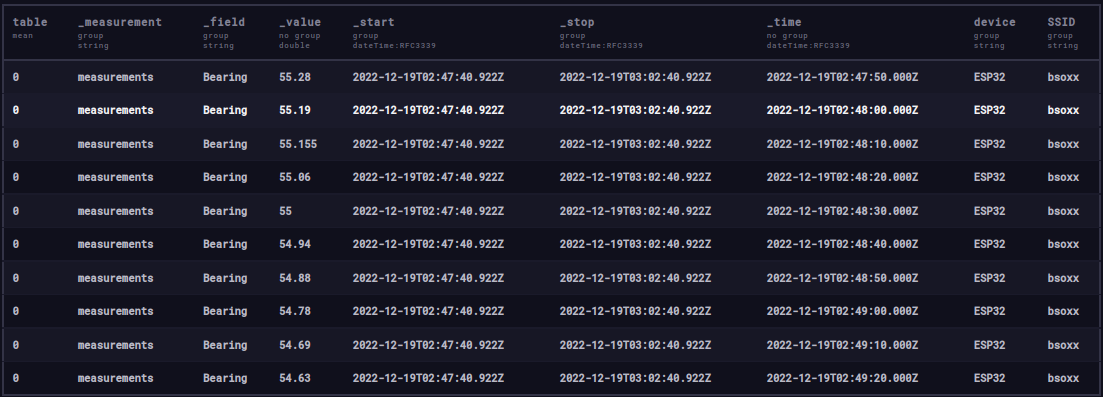
\includegraphics[width=1.0\linewidth]{Figures/csvdataset}
	\caption{Dataset}
\end{figure}
 \pagebreak
Time series data is unique because it is ordered and often exhibits serial dependence, where the value of a data point at one time is influenced by another data point at a different time. While all events happen in a sequence, time series data specifically focuses on events whose value is affected by the passage of time. This type of data can have a very high level of granularity, such as at the microsecond or nanosecond level, and the main focus is on how the values change over time.

To determine whether a given dataset is time series data, you should consider what is needed to uniquely identify a record in the dataset. Time series data consists of a series of data points that are collected at regular intervals over a period of time. These data points typically include a timestamp, which indicates when the data was collected, and one or more variables that represent the values being measured at that time. To determine whether a dataset is time series data, you will need to determine whether it includes timestamps and whether the data points are collected at regular intervals. If the dataset meets these criteria, it is likely time series data. 

At this early point it is important that the parameters remain constant. While there is a variety of reasons that cause this fluctuations we can forecast long enough and accurate enough to respond to them and thus prevent downtime.

We then monitor the residuals and set alerts when the data deviates from the forecast as shown below

Forecasts are generated for each point of data in the algorithm, which can appear to be a copy of the raw data. However, if you examine the final data point in the top graph, you will see that the forecast predicts that the temperature will continue to drop taking a steep descent towards the bottom right of the graph. This prediction is a result of the recent decrease in temperature, which is indicated by the first anomaly.

\pagebreak
 General query format . Specify time constraints then filter network name and tags to return values required.
 \begin{lstlisting}
 	from(bucket: "kk_nk")
 	|> range(start: v.timeRangeStart, stop: v.timeRangeStop)
 	|> filter(fn: (r) => r["SSID"] == "bsoxx")
 	|> filter(fn: (r) => r["_field"] == "Temperature")
 	|> filter(fn: (r) => r["_measurement"] == "measurements")
 	|> aggregateWindow(every: v.windowPeriod, fn: mean, createEmpty: false)
 	|> yield(name: "mean
 \end{lstlisting}
 
\begin{figure}[!h]
	%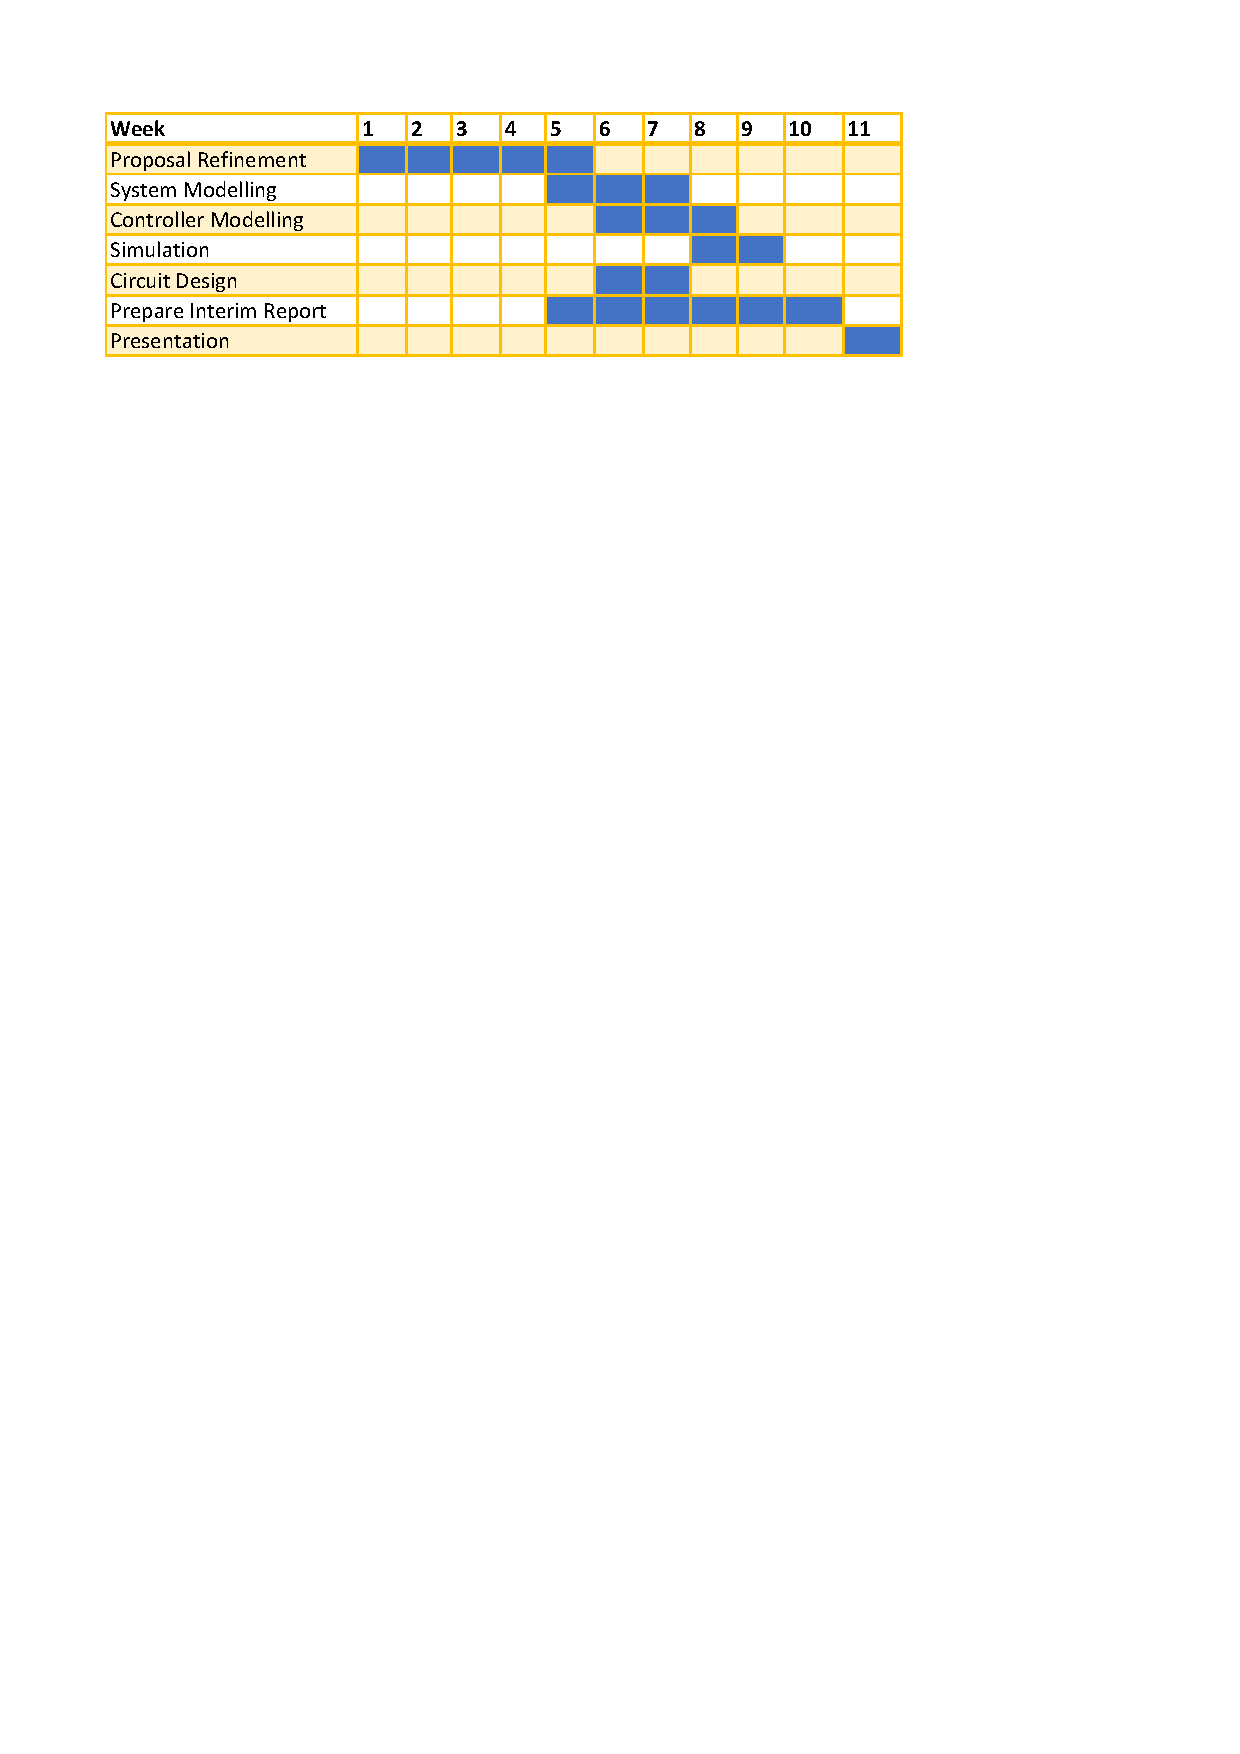
\includegraphics{Figures/workplan}
	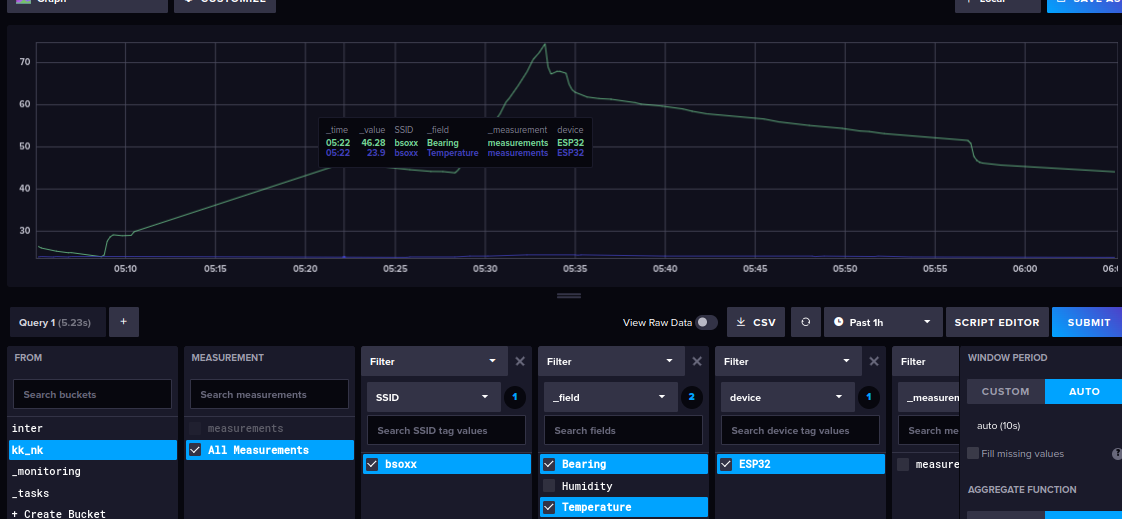
\includegraphics[width=1.0\linewidth]{Figures/dataquerying}
	\caption{Data-query example}
\end{figure}

\pagebreak
Motor performance is influenced by three factors: the voltage across the terminals, the resistance across the terminals, and the magnetic force. , we  explore how temperature and current  can affect these elements and modify motor conditions, using specific proven failure modes 

The following graph shows a benchmark values of a motor running in pristine condition




\begin{figure}[!h]
	%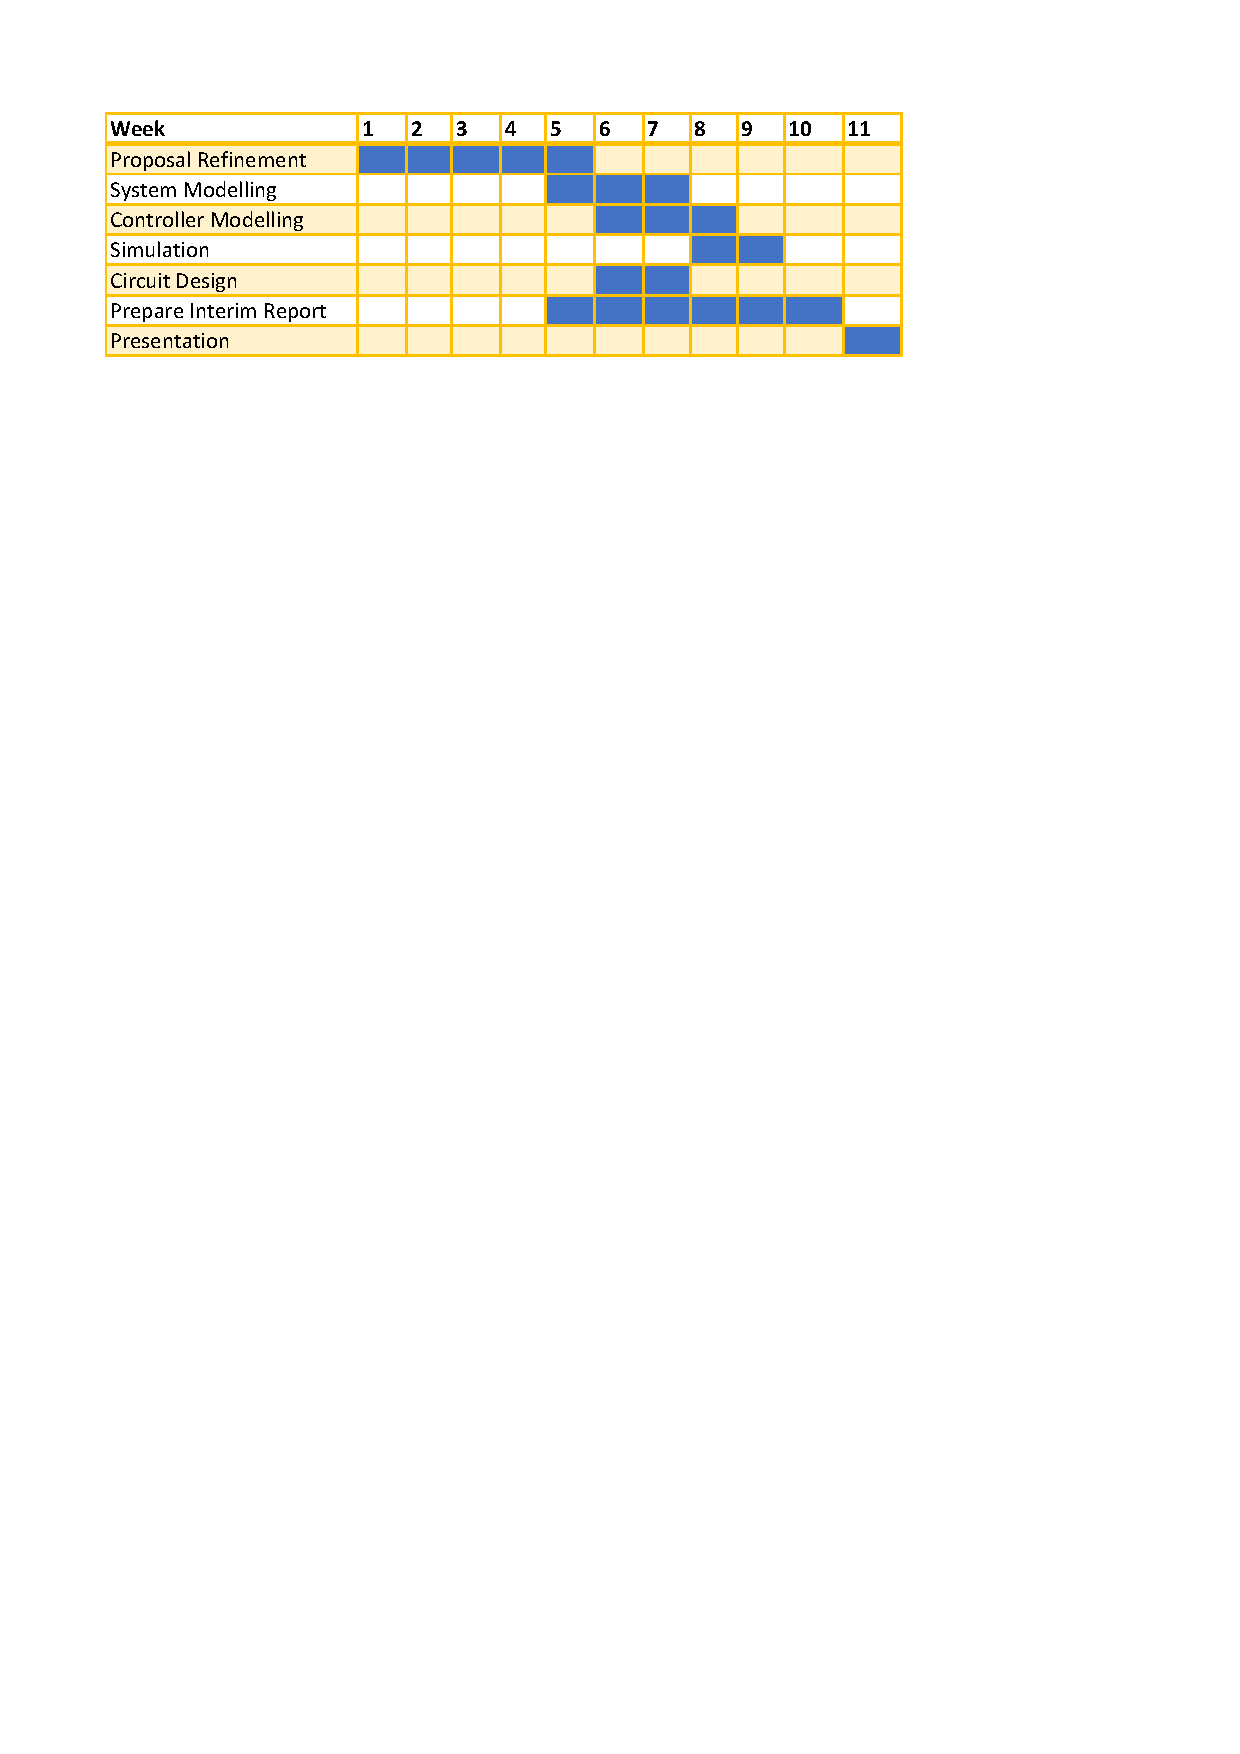
\includegraphics{Figures/workplan}
	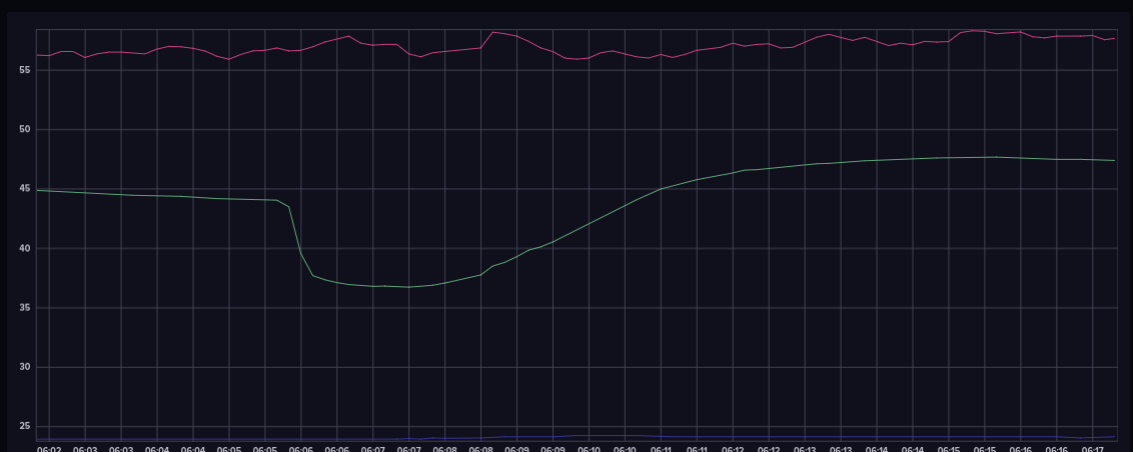
\includegraphics[width=1.0\linewidth]{Figures/normal_motor}
	\caption{Motor1}
\end{figure}

\pagebreak

Overheating motor: Quite conclusively Thermal effects on four performance characteristics of a motor:

No-load speed
As the temperature increases, the magnetic force of the magnets becomes weaker, causing N0 to rise in inverse proportion.

No-load current
The current changes in inverse proportion to the magnetic force of the magnets, but is also affected by the loss in bearing oil viscosity due to the rising temperature.

Stall current
As the temperature rises, the winding resistance decreases, causing Is to fall in inverse proportion.

Stall torque
As the temperature increases, the magnetic force of the magnets becomes weaker due to the decreasing current, causing Ts to fall greatly.


\textbf{this is clearly shown at 70 + degrees where the motor shuts down until it cools down}



\begin{figure}[!h]
	%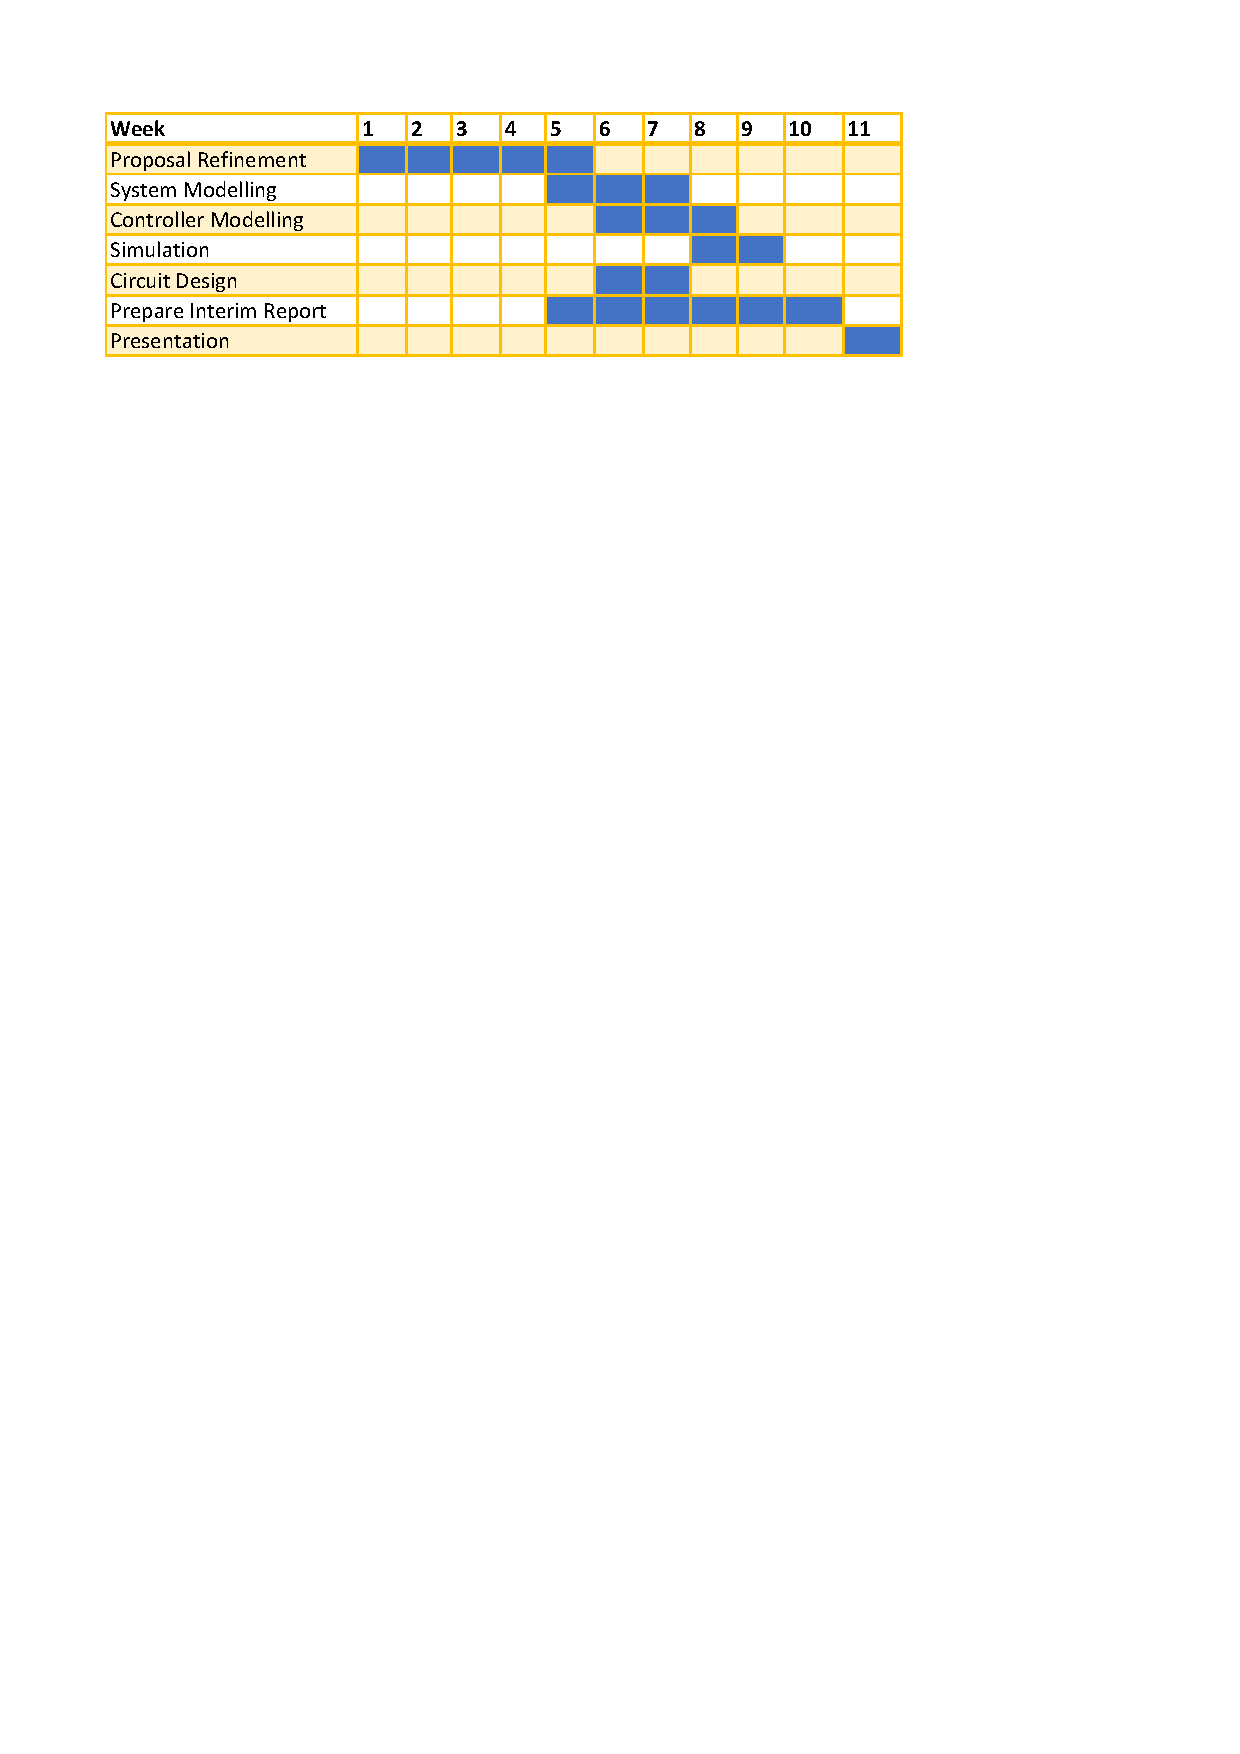
\includegraphics{Figures/workplan}
	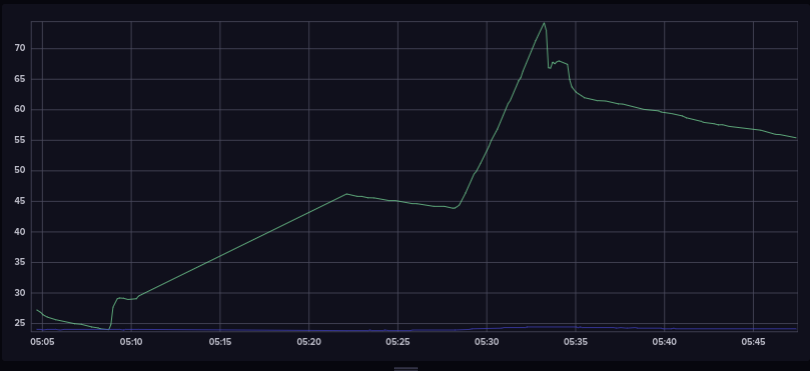
\includegraphics[width=1.0\linewidth]{Figures/overheating_motor}
	\caption{Motor3}
\end{figure}

\pagebreak

 The following graph shows the difference in operating conditions of similar motors but with different remaining useful life and how data brings out stark differences!


\begin{figure}[!h]
	%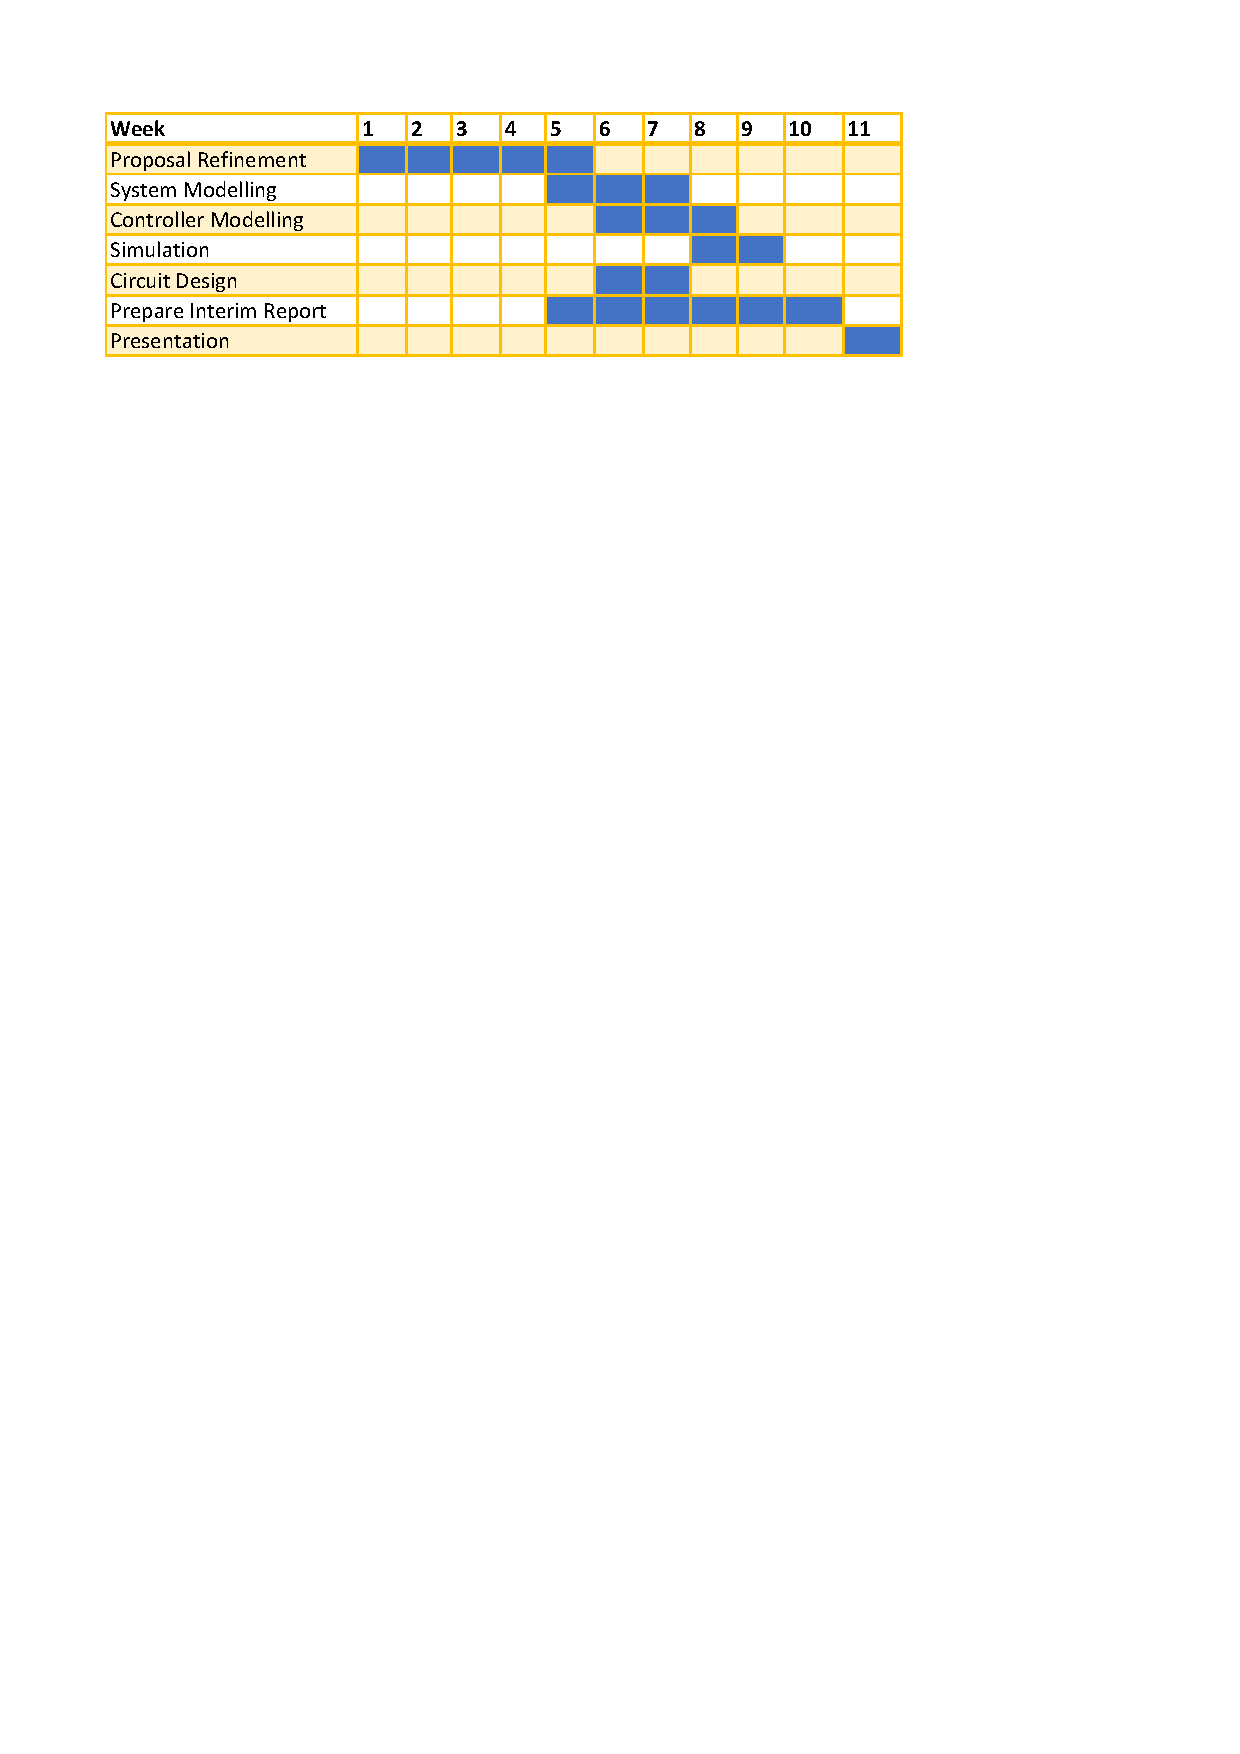
\includegraphics{Figures/workplan}
	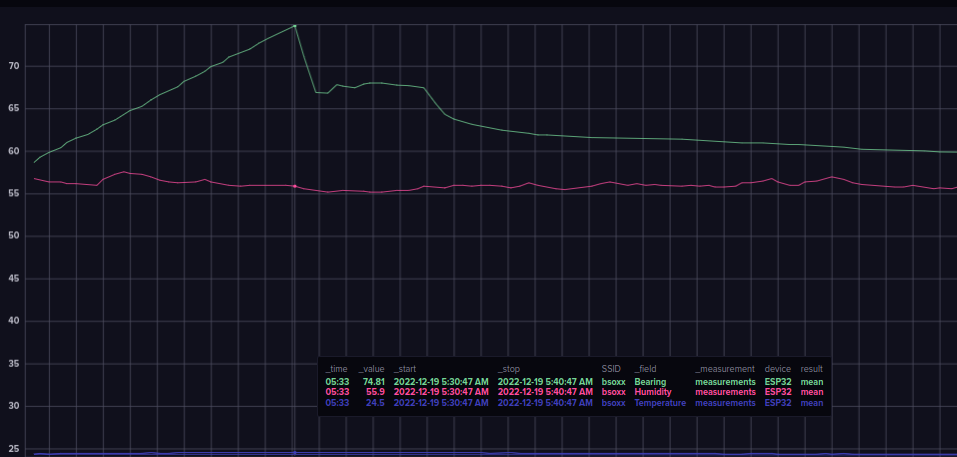
\includegraphics[width=1.0\linewidth]{Figures/normal_overheating}
	\caption{Motor comparison}
\end{figure}

\pagebreak
\begin{figure}[!h]
	%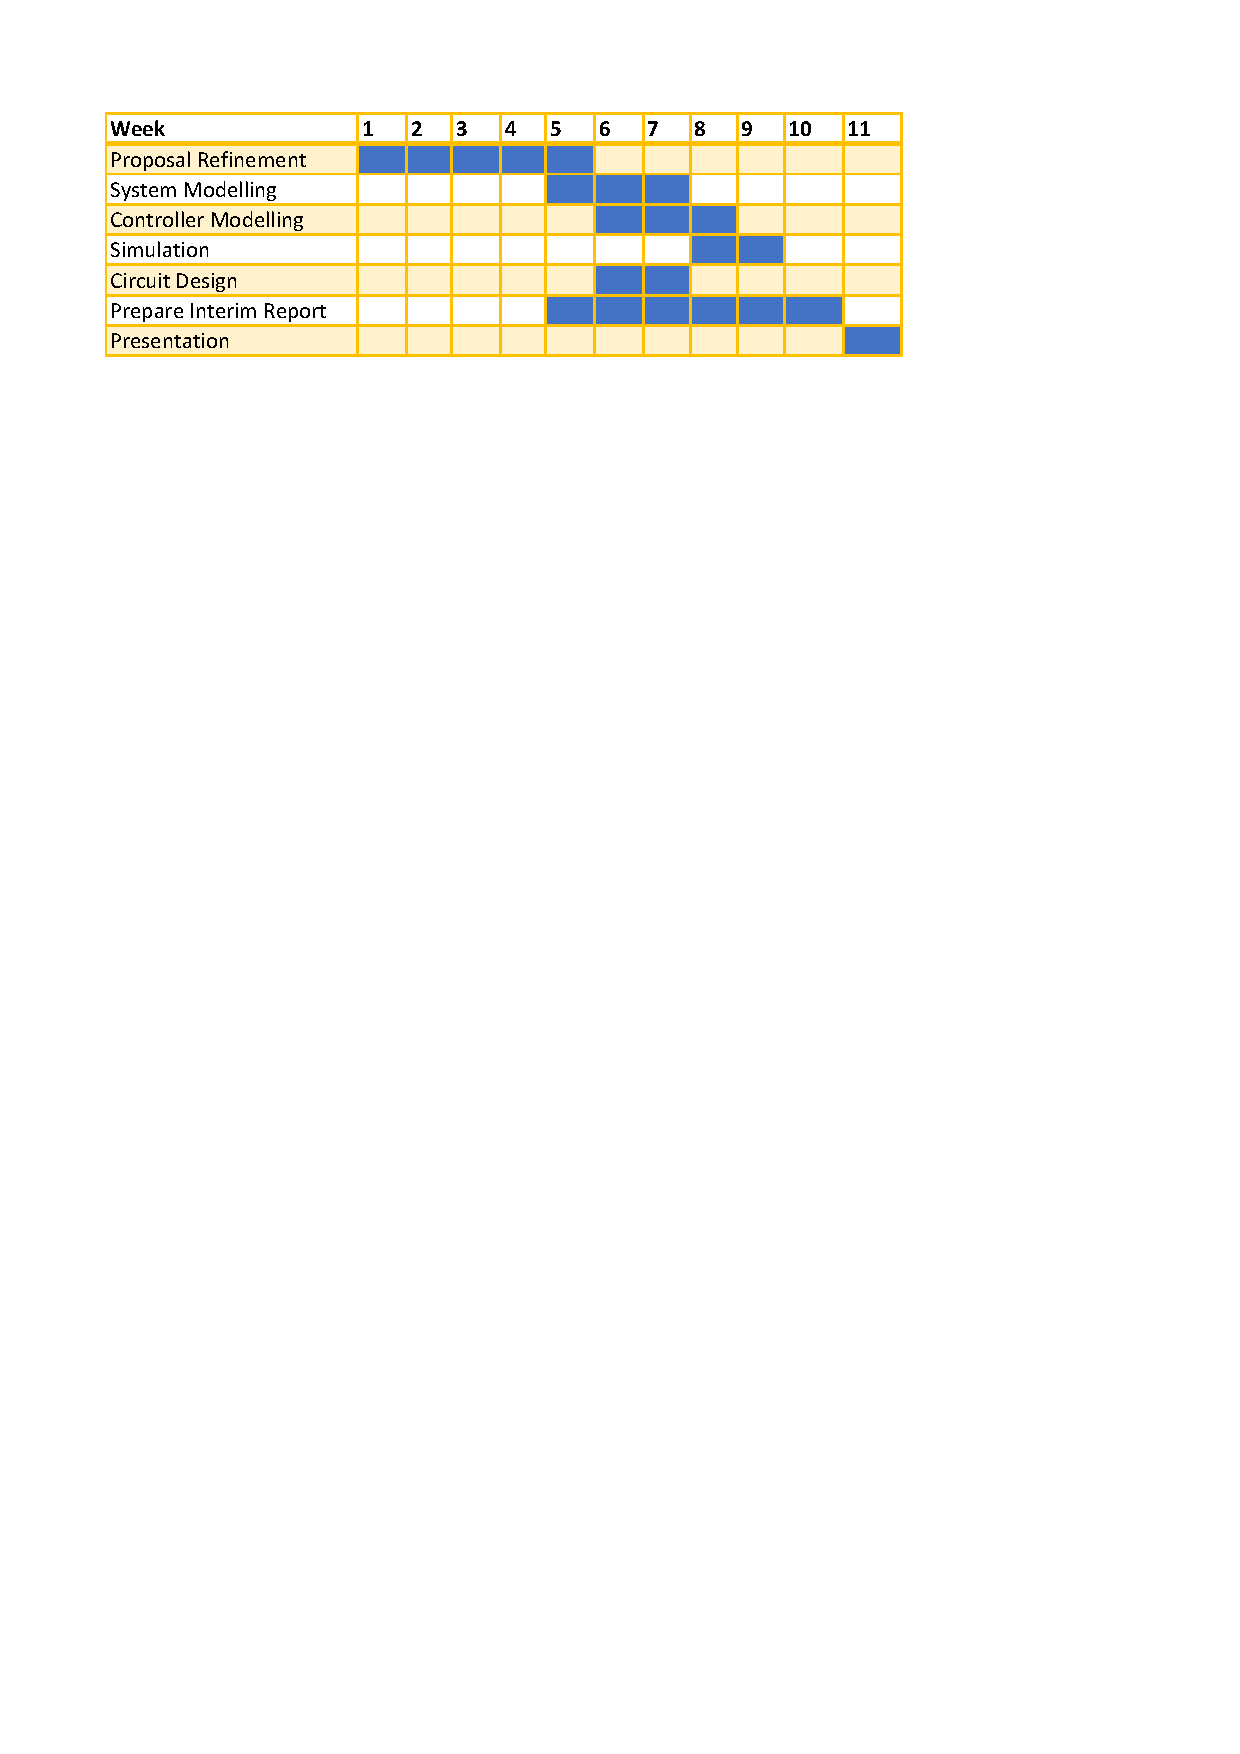
\includegraphics{Figures/workplan}
	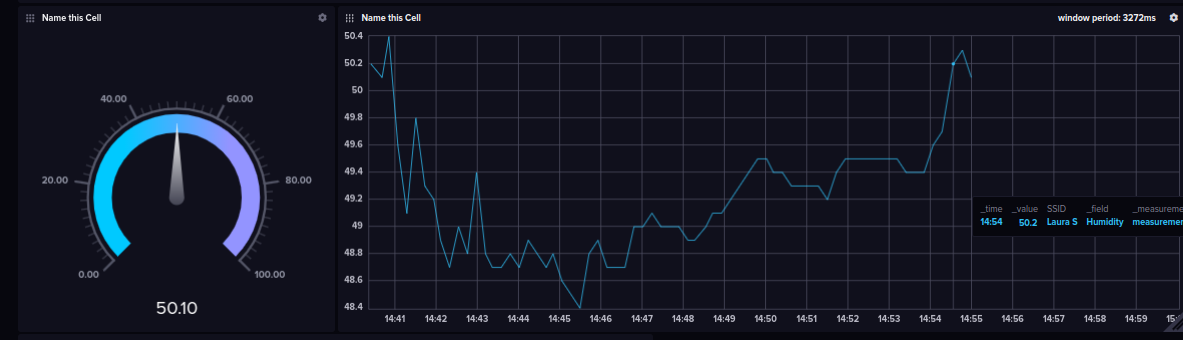
\includegraphics[width=1.0\linewidth]{Figures/remote_monitoring}
	\caption{Remote user dashboard}
\end{figure}
To set alarm and checks for automated responses from the system the following script is adjusted to motor operating conditions. where r.level indicates value of the check . eg sound  alarm when bearing temperature is above maximum operating temperature.

\paragraph*{}

Visually engaging dashboards can then be created from the data to give indicative overviews so as to require less skill in identifying critical incidents.

\begin{lstlisting}
	Check: ${ r._check_name } is: ${ r._level }
\end{lstlisting}





